\documentclass[../relazione.tex]{subfiles}

\begin{document}
\section{Progettazione}
	\subsection{XHTML}
	\begin{itemize}
		\item Logo come background tramite \textit{image replacement} affinché possa costituire informazione per il motore di ricerca (Best practice)
		\item il path svolge sia funzione di breadcrumb che di titolo della pagina, per siti che hanno un solo livello profondità non serve breadcrumb
		\item Termini caratteristici usato "strong" per indicarne l'importanza al motore di ricerca, operazione di SEO (Search Engine Optimization)
		\item struttura di ogni pagina è stata pensata per evidenziare le informazioni che si ritengono più importanti per un utente che naviga su un sito di ristorazione, quindi si è tenuto in alto il luogo (con link ad indicazioni più precise, sezione "Dove siamo" del sito) ed il numero di telefono (con il link a "tel:"), visibili in ogni pagina
		\item index.html: in evidenza: orario, le informazioni generali riguardo il ristorante e la possibilità di usufruire del servizio di asporto
		\item chi-siamo.html: per fidelizzare il cliente mostrando le personalità principali che gestiscono l'attività come il proprietario del ristorante e i cuochi, indicando o un sunto del loro curriculum o le loro esperienza passate nel campo della ristorazione
		\item dove-siamo.html: una breve descrizione testuale accompagnata da un'immagine che indica la posizione del ristorante rispetto ai vicini punti di interesse. Per rendere accessibile l'immagine a chi utilizza uno screen reader è stato utilizzato l'attributo "longdesc" per l'immagine che associa una descrizione testuale estesa alle informazioni visive fornite dall'immagine. Oltre a questo, è presente un link a Google Maps per agevolare l'utente nella ricerca di indicazioni precise per raggiungere il ristorante: nel caso in cui stia navigando da un dispositivo mobile ed abbia l'applicazione di Google Maps installata, verrà automaticamente lanciata l'applicazione.
		\item curiosita.html: per far conoscere all'utente un po' di storia della cucina giapponese
		\item menu.cgi: tutti i nomi delle pietanze sono inseriti in un tag "strong" per indicarne l'importanza al motore di ricerca, operazione di SEO (Search Engine Optimization)
		\item Area amministratore: permette di aggiungere, modificare o rimuovere pietanze o bevande dal menù
	\end{itemize}
	\subsection{CSS}
	\begin{itemize}
		\item si è cercato di utilizzare meno colori possibili
		\item si è scelto di utilizzare i colori di bandiera del ristorante, ricavati dal logo fornitoci dal proprietario del ristorante
		\item tali colori sono stati scelti antagonisti, per venire incontro a utenti con problemi di colorblindness ed aumentando così l'accessibilità del sito
		\item Lo sfondo in legno dell'intero sito web vuole ricordare la stuoia usata nel processo di creazione del sushi e, più in generale, lo stile nipponico.
	\end{itemize}
	\subsection{Perl/CGI}
	\begin{itemize}
		\item 
	\end{itemize}
	\subsection{Javascript}
	\begin{itemize}
		\item Nav inizialmente visibile, così se non c'è JS ho degradazione elegante. Se JS funziona, allora viene nascosto e rimane accessibile dall'apposito bottone
		\item è presente il controllo dei dati inseriti nei campi nelle form di login, aggiunta e modifica
		\item il menù è diviso in categorie inizialmente chiuse per diminuire la lunghezza della pagina e dare all'utente una visione generale delle categorie di pietanze presenti nel menù
		\item nel caso in cui il Javascript sia disattivato, il menù verrà mostrato per intero, ma viene aggiunta una funzionalità di ricerca veloce in alto e, alla fine di ogni categoria, un ancora per tornare all'inizio della pagina
	\end{itemize}
	\subsection{XML e XMLSchema}
	\begin{itemize}
		\item 
	\end{itemize}
	\subsection{Mobile}
	riportare motivi per cui è stata implementata anche la versione mobile
	\begin{itemize}
		\item menù può essere accessibile da mobile
		\item usato la "hamburger icon", ritenuta adeguata perché ormai consuetudine per gli utenti associare ad essa il menu del sito
		\item abbiamo pensato che fosse comodo per l'utente poter aprire e chiudere il menu del sito (nav), per agevolare la visita del sito, per rendere più piacevole l'esperienza: per far ciò è stata utilizzata una funzione Javascript che mostra e nasconde il nav attraverso l'icona hamburger
		\item abbiamo convenuto che la parte mobile sia dedicata interamente agli utenti, quindi abbiamo impedito l'accesso all'area amministratore da mobile, esso è permesso solo da desktop
		\item il sito è stato testato sui seguenti browser mobile: Google Chrome, Safari
	\end{itemize}
	\begin{figure}[H]
		\centering
		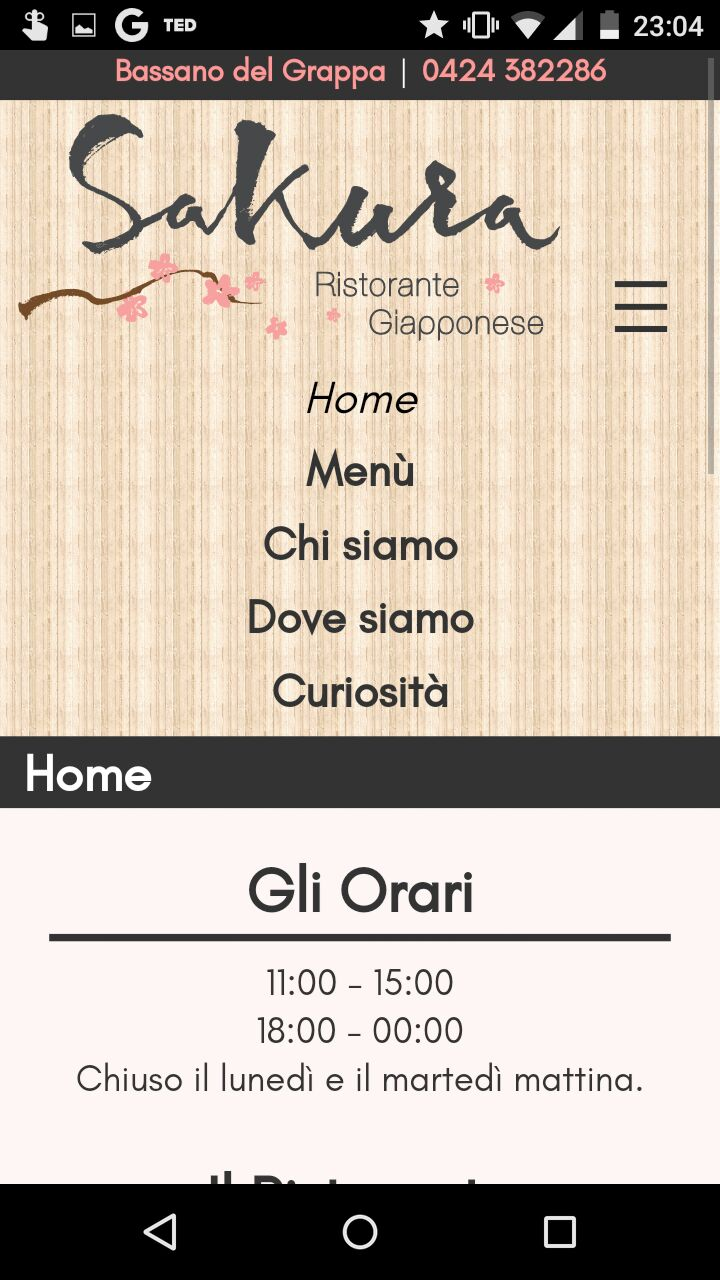
\includegraphics[scale=0.2]{images/mobile2}
		\caption{Esempio di pagina vista da dispositivo mobile}
		\label{fig:Esempio di pagina vista da dispositivo mobile}
	\end{figure}
\end{document}